
%%%
% Any line that begins with a percent symbol is a comment. To compile
% this document and view the output:
%
% Run Latex
% Run Bibtex
% Then run Latex twice.
%
% This should produce the output PDF file named main.pdf
%%%

% This defines the style to use for this document.
% Do not modify.
\documentclass[letterpaper]{article}

% The following are akin to "import" statements in Python or Java -
% these import useful commands into the document for you to use.  You
% don't have to modify any of these lines. The AAAI package formats
% this document in the style of submissions to the American
% Association for Artificial Intelligence conference, one of the top
% AI conferences in the world. You will find that many academic
% publications in AI use this format.
\usepackage{aaai} 
\usepackage{times} 
\usepackage{helvet} 
\usepackage{courier} 
\setlength{\pdfpagewidth}{8.5in} 
\setlength{\pdfpageheight}{11in} 
\usepackage{amsmath}
\usepackage{amsthm}
\usepackage{graphicx}
\usepackage{graphics}
\usepackage{moreverb}
\usepackage{subfigure}
\usepackage{epsfig}
\usepackage{txfonts}
\usepackage{algpseudocode}
\usepackage{multirow, multicol}
\usepackage{url}
\usepackage{tablefootnote}
\usepackage{color}

\setcounter{secnumdepth}{1}
\nocopyright

% Fill in your paper title, names and emails below
% The "\\" is used to break lines. The \url command
% is useful for typesetting URLs and email addresses (it uses the
% Courier font).
\title{Solving the 8-Puzzle}
 \author{Alan Turing \and John von Neumann\\
 \url{{alturing, jovonneumann}@davidson.edu}\\
 Davidson College\\
 Davidson, NC 28035\\
 U.S.A.}

% This is the "true" start of the document. All the text in your
% write-up should be placed within the \begin{document} and
% \end{document} decorators.
\begin{document}

\maketitle % formats the title nicely, do not modify

% While at this point you could just begin your write-up, often, it's
% useful to write each section of your write-up in a separate tex
% file (not unlike the modular decomposition you do for code you
% write). These \input commands insert the contents of the
% specified tex files in the order specified. Every write-up you
% submit must contain the following sections, in the shown order. Open
% each of the indicated tex files to understand what goes in each
% section, as well as for more TeX tips.
% Place the contents of your abstract between the
% \begin{abstract} and \end{abstract} decorators.

\begin{abstract}
This is a machine learning project that focused on predicting the quality of red and white wine using existing datasets. In this project, we will train, validate, and test four regression models: the linear regression model, the SGD (Stochastic Gradient Descent) model, the Ridge model (L-2 norm), and the Lasso model (L-1 norm). After conducting series of experiments on these models, we rank their performances based on the results of wine quality prediction. Our analysis shows that Ridge gives the highest score, outperforming the other three, for both red and white wine. We think such model can be useful to support educational wine tasting activities to improve wine production, and can help businesses better understand consumer needs.
 \textbf{Do \emph{not}
include any citations in the abstract.}



% The \textbf{} command makes the specified text bold. The \emph{} or
% \textit{} command are used to italicize text. In general, text is never
% underlined.

% DON'T FORGET TO MATCH EACH OPEN BRACE WITH A CLOSING BRACE!
\end{abstract}


% The \section{} command formats and sets the title of this
% section. We'll deal with labels later.
\section{Introduction}
\label{sec:intro}
Wine is one of the most popular alcoholic beverages in the world, and the wine industry is a multi-billion dollar industry that boosts the economy of a number of US states. With the thousands of varieties of wine on the market currently, an important question arises: Which one should you buy? Wine experts can of course rate the quality of a wine, but the average consumer does not always have easy access to such expertise. In this paper, we attempt to predict the quality of a wine given a number of its physicochemical properties using datasets from Cortez et al.(2009). A machine learning algorithm that could accurately predict the quality of a wine given some of its features could be instrumental in bringing the capability to evaluate the quality of wine to consumers that don't have any special training.\\

Our dataset consists of two files, \path{winequality-red.csv} and \path{winequality-white.csv}, containing red wine and white wine data respectively. The red wine dataset includes information about $1599$ wines, and the white wine dataset includes information about $4898$ wines. The type of information included in both datasets is the same. A quality column holds information about the quality of wine as rated by wine experts who rated the quality of each wine between $0$(very bad) and $10$(very excellent). This quality data is what we are interested in predicting, and will henceforth be referred to as the target variable. The datasets also include columns that detail information regarding the fixed acidity, volatile acidity, citric acid, residual sugar, chlorides, free sulfur dioxide, total sulfur dioxide, density, pH, sulphates, and alcohol content of each wine. These 11 variables make up the set of features that will be used to predict the target or the quality. The features are all in floating point format while the target is in integer format.\\

Next, we will provide a brief explanation of the models we used while solving this problem and also provide an overview of the preprocessing that the data goes through. Following that, we will conclude by summarizing the performance of our models, and comparing and analyzing the results.\\





\section{Background}
\label{sec:background}
Given that this is our first project for this class, we decided to stick mostly to models that had been mentioned in class. As such, we tried out the linear regression, stochastic gradient descent (SGD), ridge regression, and LASSO models from the Python \texttt{scikit-learn} library. We also tried a stochastic gradient descent classification model, \texttt{SGDClassifier}, from the same library as well.
\begin{itemize}
    \item \textbf{Linear regression} - A straightforward model that focuses on finding the weights associated with the least cost in a linear combination of the features of the dataset. 
    \item \textbf{SGD} - Similar to linear regression, except the entire set of training examples is not evaluated each time a decision about minimizing the cost function is made. Instead, a random training example is chosen, and the minimum point of the cost function is calculated using that randomly chosen training example.
    \item \textbf{Ridge regression} - A version of linear regression that employs an L-2 regularization strategy. Ridge regression regulates the complexity of the curve used to fit the data by employing a penalty for higher weights. The specific penalty used is called the L-2 penalty and is defined as $\sum_{j=1}^{n} \theta_{j}^{2}$.
    \item \textbf{LASSO} - Similar to ridge regression, except the regularization penalty used is L-1, which is defined as $\sum_{j=1}^{n} |\theta_{j}|$.
    \item \textbf{SGDClassifier} - While this model was not talked about in class, it is similar to the regular SGD model in that gradient descent updates are made using single or batches of training examples instead of the whole dataset. However, a major difference is that \textt{SGDClassifier} is used for classification problems. A classification problem is any problem where the target variable can only take on a finite set of discrete values. Since our target variable, quality, can only take on values from 0 to 10 (inclusive), this problem can also be classified as a classification problem. \texttt{SGDClassifier} also makes use of a regularization penalty.
\end{itemize}
Before any of these models could be run, however, it was necessary that the data went through some preprocessing. We used the \texttt{pandas} Python library to import the data from the files and store them with the appropriate column headers. We used one file to house all the functions needed to preprocess the data, which we called \path{winequality.py}. This file held the \path{read_file}, \path{select_features}, \path{make_poly}, \path{standardize}, \path{drop_outliers}, \path{split}, \path{get_XY}, and \path{get_preprocessed_dataset} functions. 
\begin{enumerate}
    \item The \path{read_file} function was used to read in the .csv file and store it in a DataFrame object.
    \item Then, we split the file into the features and the quality, so that we could easily apply some preprocessing functions only to the features dataset.
    \item The \path{select_features} function was used to trim down the dataset to only the features we wanted to train the models with. The way we decided which features to use will be explained shortly.
    \item The \path{make_poly} function used \texttt{PolynomialFeatures} that was also imported from the \texttt{scikit-learn} library. We used \texttt{PolynomialFeatures} to add extra columns to the dataset to simulate higher-order polynomials.
    \item Then, we used the \path{standardize} function to standardize the dataset using \textt{StandardScaler} from the \texttt{scikit-learn} library.
    \item The standardized DataFrame had the quality variable added back in and then we dropped all outliers from the dataset. The \path{drop_outliers} function dropped any outliers that weren't within $3$ standard deviations of the mean of any column.
    \item The \path{split} function split the dataset into a 60-20-20 split to represent the training, validation, and testing datasets.
\end{enumerate}      
The \path{get_XY} function accepted a DataFrame as input and returned the features and the target separately. Finally, \path{get_preprocessed_dataset} was a master function that called all of the other functions and returned the preprocessed dataset.\\

To begin the process of feature engineering, we ran some statistical analyses on our datasets. First, we created graphs of quality vs. each feature to see if there were any outliers. A few of the graphs showed some data points that were considerably different from any others (see Figure 1). For example, the citric acid value for entry $152$ of the red wine dataset was $3.7$ standard deviations above the mean for citric acid. According to Wilcox (2001), even a single outlier can mask an otherwise strong correlation between the predictor and the criterion for Pearson's correlation. Keeping this in mind, we decided to drop all outliers from our datasets.\\
\begin{figure}[htb]

  \centering  % centers the image in the column

  % replace the second argument below with your filename. I like to
  % place all my figures in a sub-directory to keep things organized
  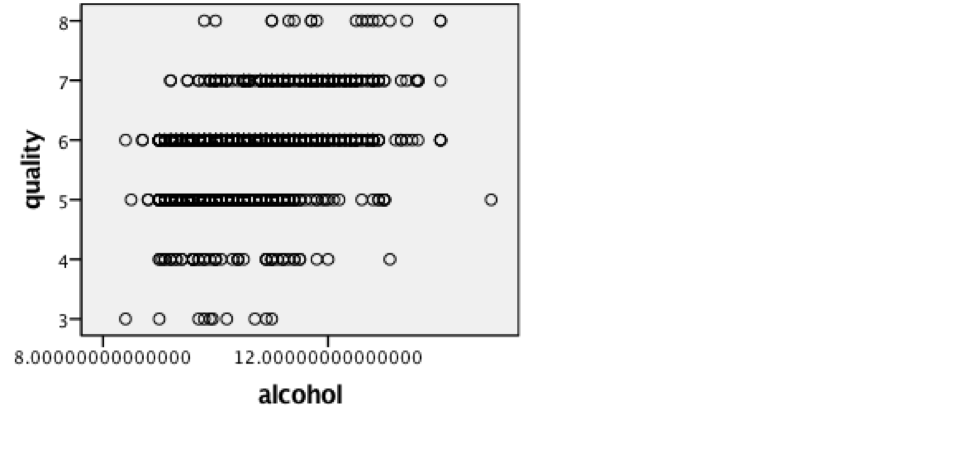
\includegraphics[width=0.47\textwidth]{Picture2.png}

  % *Every* figure should have a descriptive caption.
  \caption{Correlation Between Alcohol and Quality}

  % The label is a handle you create so that you can refer to this
  % figure (using the \ref{} command) from other parts of your
  % document. LaTeX automatically renumbers figures and updates
  % references when you recompile, so you should do it this way rather
  % than hard-coding in references. Notice that I've also been
  % creating labels for the various sections in the document; I could
  % use \ref{} command to refer to those sections using their labels
  % too.
  \label{fig:tex}

  \end{figure}
  
  \begin{figure}[htb]

  \centering  % centers the image in the column

  % replace the second argument below with your filename. I like to
  % place all my figures in a sub-directory to keep things organized
  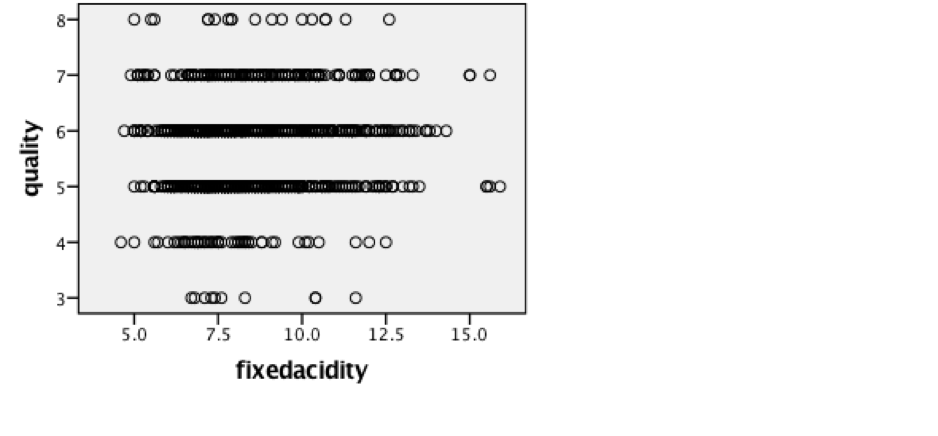
\includegraphics[width=0.47\textwidth]{Picture1.png}

  % *Every* figure should have a descriptive caption.
  \caption{Correlation Between Fixed Acidity and Quality}

  % The label is a handle you create so that you can refer to this
  % figure (using the \ref{} command) from other parts of your
  % document. LaTeX automatically renumbers figures and updates
  % references when you recompile, so you should do it this way rather
  % than hard-coding in references. Notice that I've also been
  % creating labels for the various sections in the document; I could
  % use \ref{} command to refer to those sections using their labels
  % too.
  \label{fig:tex}

  \end{figure}
   \begin{figure}[htb]

  \centering  % centers the image in the column

  % replace the second argument below with your filename. I like to
  % place all my figures in a sub-directory to keep things organized
  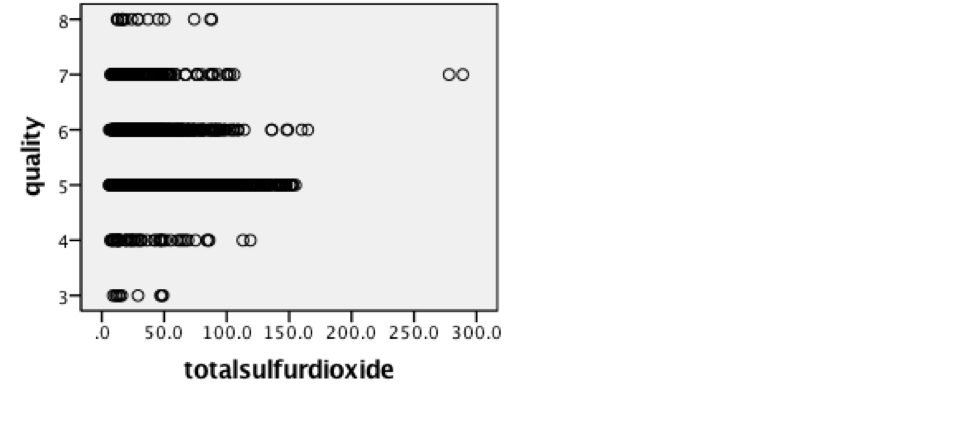
\includegraphics[width=0.47\textwidth]{3.png}

  % *Every* figure should have a descriptive caption.
  \caption{Correlation Between Total Sulfur Dioxide and Quality}

  % The label is a handle you create so that you can refer to this
  % figure (using the \ref{} command) from other parts of your
  % document. LaTeX automatically renumbers figures and updates
  % references when you recompile, so you should do it this way rather
  % than hard-coding in references. Notice that I've also been
  % creating labels for the various sections in the document; I could
  % use \ref{} command to refer to those sections using their labels
  % too.
  \label{fig:tex}

  \end{figure}
  
  
The next step in deciding which features were most important, we computed a Pearson's correlation coefficient between each feature and quality for each dataset. Figures 4 and 5 contain the correlation coefficients we computed, ordered from the strongest to the weakest. We discovered that pH, free sulfur dioxide, and residual sugar showed the weakest correlations with quality for the red wine dataset. Sulphates, citric acid, and free sulfur dioxide showed the weakest correlations with quality for the white wine dataset. Given these results, we ran some experiments excluding some of these features that were weakly correlated with quality. A summary of our experiments and results is provided in the next two sections.
\begin{figure}[htb]
  \centering % centers the entire table

  % The following line sets the parameters of the table: we'll have
  % three columns (one per 'c'), each
  % column will be centered (hence the 'c'; 'l' or 'r' will left or
  % right justify the column) and the columns
  % will have lines between them (that's the purpose of the |s between
  % the 'c's).
 \begin{tabular}{|c|c|} 
   \hline \hline % draws two horizontal lines at the top of the table
    Feature & Correlation with Quality \\ % separate column contents using the &
    \hline % line after the column headers
    Alcohol & $0.476$** \\
     \hline
    Volatile Acidity & $-0.391$** \\
     \hline
    Sulphates & $0.251$** \\
     \hline
    Citric Acid   & $0.226$** \\
     \hline
    Total Sulfur Dioxide  & $-0.185$** \\
     \hline
    Density  & $-0.175$** \\
     \hline
    Chlorides & $-0.129$** \\
     \hline
    Fixed Acidity  & $0.124$** \\
     \hline
    pH  & $-0.058$* \\
     \hline
    Free Sulfur Dioxide    & $0.051$* \\
     \hline
    Residual Sugar   & $0.014$ \\
  
    \hline \hline  
    \end{tabular}
  % As with figures, *every* table should have a descriptive caption
  % and a label for ease of reference.
  \caption{Feature Correlation with Quality for Red Wine}
  \label{tab:example}

\end{figure}

  \begin{figure}[htb]
  \centering % centers the entire table

  % The following line sets the parameters of the table: we'll have
  % three columns (one per 'c'), each
  % column will be centered (hence the 'c'; 'l' or 'r' will left or
  % right justify the column) and the columns
  % will have lines between them (that's the purpose of the |s between
  % the 'c's).
 \begin{tabular}{|c|c|} 
   \hline \hline % draws two horizontal lines at the top of the table
    Feature & Correlation with Quality \\ % separate column contents using the &
    \hline % line after the column headers
    Alcohol & $0.436$** \\
     \hline
    Density & $-0.307$** \\
     \hline
    Chlorides & $-0.210$** \\
     \hline
    Volatile Acidity   & $-0.195$** \\
     \hline
    Total Sulfur Dioxide  & $-0.175$** \\
     \hline
    Fixed Acidity  & $-0.114$** \\
     \hline
    pH & $0.099$** \\
     \hline
    Residual Sugar & $-0.098$** \\
     \hline
    Sulphates  & $0.054$** \\
     \hline
    Citric acid   & $-0.009$ \\
     \hline
    Free Sulfur Dioxide  & $0.008$ \\
  
    \hline \hline  
    \end{tabular}
  % As with figures, *every* table should have a descriptive caption
  % and a label for ease of reference.
  \caption{Feature Correlation with Quality for White Wine}
  \label{tab:example}


\end{figure}






\section{Experiments}
\label{sec:expts}

The steps we followed while conducting our experiments are detailed below:
\begin{enumerate}
    \item All of our models were housed in separate files. Each model imported their respective model files from the \texttt{scikit-learn} library, and the \path{get_preprocessed_dataset} and \path{get_XY} functions from \path{winequality.py}. Some models made use of other functions that will be detailed later in this section. All models were run using a \path{run_model} function that we wrote to fetch the preprocessed dataset, train the model, and report the $R^2$ score for the model using the model's \texttt{score} function. All models were run $50$ times and the final $R^2$ scores reported in this paper are the average of $50$ runs.
    \item Initially, we ran all models using their default settings, and also using all the features in the dataset. The results we got served as our baseline results, so any time we modified our models, we could see if they did better or worse. After the initial step, we decided to add the \path{drop_outliers} function to the preprocessing step. Based on the graph of correlations between feature variables and quality scores, we observed a few outlier feature scores that were more than $3$ standard deviations away from the mean. The performance scores for all models improved in a small but consistent manner after these outliers were dropped.
    \item Next, we decided to tune hyperparameters to increase the performance of our models. We used \texttt{GridSearchCV} from the \texttt{scikit-learn} library to do this. \texttt{GridSearchCV} not only uses grid search to try different combinations of hyperparameters, but it also uses cross-validation when training and testing the models. For our SGD model, we varied \textbf{alpha}, a constant that multiplies the regularization term, over [0.00001, 0.00002, 0.00005, 0.0001]. We also varied \textbf{eta0}, the learning rate of the model, over [0.001, 0.002, 0.005, 0.01]. We also varied \textbf{alpha} for ridge regression over [0.01, 0.02, 0.05, 0.1, 0.2, 0.5, 1.0, 2.0, 5.0, 10.0]. For the LASSO model, we varied \textbf{alpha} over [0.01, 0.02, 0.05, 0.1, 0.2, 0.5, 1.0]. Finally, for the SGD classifier model, we varied \textbf{eta0} over [0.001, 0.002, 0.005, 0.01], and \textbf{alpha} over [0.00001, 0.00002, 0.00005, 0.0001]. \texttt{GridSearchCV} resulted in increased scores for all the models.
    \item We were curious whether increasing the complexity of the model would improve the scores, so we decided to adopt the \texttt{PolynomialFeatures} function from the \path{scikit-learn} library. This feature generates new feature columns consisting of all polynomial combinations of the features with degree less than or equal to the specified degree. After trying to increase degrees to $2$,$3$,and $4$, we observed that a polynomial degree of $2$ gave the best performance for all models, and scores started to deteriorate for models with degrees higher than $2$.
    \item Finally, we used feature selection/elimination in an effort to improve the performance of our models. Using the dataset, we generated a series of analyses using SPSSStatistics on correlations between individual feature variables and quality scores. We then ranked correlations from highest to lowest for both red and white wine, and picked the top $8$ features with the highest correlations as our default selected features. These analyses can be seen in Figures 1 and 2. For all five models, there were no significant improvements after we eliminated the least correlated two features. In addition, when we tried to eliminate more features, we noticed decreases in performance scores for all models. Thus, we decided to not eliminate any features, and include all the original features.
\end{enumerate}

Our results will be discussed in the next section.


\section{Results}
\label{sec:results}

Present the results of your experiments. Simply presenting the data is
insufficient! You need to analyze your results. What did you discover?
What is interesting about your results? Were the results what you
expected? Use appropriate visualizations. Prefer graphs and charts to
tables as they are easier to read (though tables are often more
compact, and can be a better choice if you're squeezed for space).

\subsection{Embedding Pictures}
\label{subsec:pics}

See the source code (\texttt{results.tex}) for instructions on how to
insert figures (like figure~\ref{fig:tex}) or plots into your
document.

% Note that TeX has a mind of its own when it comes to placing images
% in documents - where a figure appears in the PDF document will often
% be quite different from where it appears in the source code. This is
% a feature, not a bug - it enables LaTeX to produce layouts that
% "flow" better. It only takes a few lines to insert a figure into
% your write-up - I recommend using PNG, JPG or PDF images
% (incidentally, programs like Excel and Matlab will allow you to save
% any plots or figures you generate in those formats). The \figure{}
% command is used to create a new figure.
\begin{figure}[htb]

  \centering  % centers the image in the column

  % replace the second argument below with your filename. I like to
  % place all my figures in a sub-directory to keep things organized
  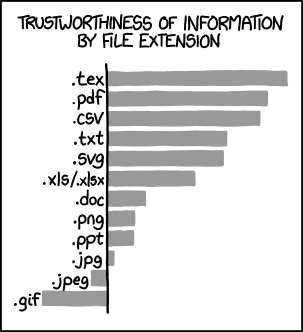
\includegraphics[width=0.47\textwidth]{figs/file_extensions.png}

  % *Every* figure should have a descriptive caption.
  \caption{On the trustworthiness of \LaTeX. Image courtesy of \texttt{xkcd}.}

  % The label is a handle you create so that you can refer to this
  % figure (using the \ref{} command) from other parts of your
  % document. LaTeX automatically renumbers figures and updates
  % references when you recompile, so you should do it this way rather
  % than hard-coding in references. Notice that I've also been
  % creating labels for the various sections in the document; I could
  % use \ref{} command to refer to those sections using their labels
  % too.
  \label{fig:tex}

\end{figure}

\subsection{Creating Tables}
\label{subsec:tables}

Again, refer to \texttt{results.tex} to learn how to create simple
tables (like table~\ref{tab:example}).
\begin{figure}[htb]
  \centering % centers the entire table

  % The following line sets the parameters of the table: we'll have
  % three columns (one per 'c'), each
  % column will be centered (hence the 'c'; 'l' or 'r' will left or
  % right justify the column) and the columns
  % will have lines between them (that's the purpose of the |s between
  % the 'c's).
  \begin{tabular}{|c|c|c|} 
    \hline \hline % draws two horizontal lines at the top of the table
    Column 1 & Column 2 & Column 3 \\ % separate column contents using the &
    \hline % line after the column headers
    $1$ & $3.1$ & $2.7$ \\
    $42$ & $-1$ & $1729$\\
    \hline \hline
  \end{tabular}

  % As with figures, *every* table should have a descriptive caption
  % and a label for ease of reference.
  \caption{An example table.}
  \label{tab:example}

\end{figure}



\section{Conclusions}
\label{sec:concl}

In this paper, we set out to build a model that could accurately predict the quality of wine from $11$ of its physicochemical properties. After conceptualizing, building, and training our models, we discovered that \texttt{SGDClassifer} came away with the best results, for both red and white wine. From the models that we discussed in class, the ridge regression model proved to be the best, for both red and white wine again. Our most important discovery is that using second order polynomials improved the performance of our models by a fair amount. Perhaps using second order polynomials along with some other manipulation of hyperparameters is required for this problem.\\

Although the performance of our models wasn't exactly groundbreaking, we think this is a valuable step towards the right direction. Future studies can perhaps look more deeply into feature selection as a way of improving the performance of the models. Also, we were limited by our knowledge to models we had covered in class. Perhaps other models would perform better than ours. So, even though some progress had been made, there's still time left before wine experts are replaced by computers.


\section{Contributions}
\label{sec:contrib}

Briefly summarize the contributions of you and your partner in this
section. For example: ``A.T. wrote the gradient descent code and ran
experiments; J.vN. ran the experiments using scikit-learn's built-in
regression solver. A.T. wrote the introduction and background sections
and prepared figure \ref{fig:tex} and table
\ref{tab:example}. J.vN. wrote the experiments and results
sections. Both authors proof-read the entire document.'' I will be
looking for roughly equal contributions from both partners in both
aspects of the assignment (i.e., the programming/data
preprocessing/experimentation and writing).



\section{Acknowledgements} 
\label{sec:ack} 

We would like to thank Dr. Ramanujan for his patient instructions at the beginning of our project, as well as our friends and classmates for their generous encouragement and support. 


% This creates the references section. Open the project1.bib file to
% see how to organize your references.
\bibliography{project1}
\bibliographystyle{aaai} % sets citation and bib style, do not modify

\end{document}
